\section{Beantwortung der Aufgaben des Labors zu EMG-Signalen}

\subsection{Aufgabe 1: Darstellung des Messsystems}
Das in Abbildung \ref{fig:blockschlaltbild_lab3} dargestellte Blockschaltbild veranschaulicht den
Aufbau des Messsystems zur Erfassung und Analyse von EMG-Signalen im Rahmen der Laboreinheit.
Die verwendeten Komponenten sind in Tabelle \ref{tab:verwendete_komponenten} aufgelistet und durchnummeriert.
\begin{figure}[h]
    \centering
    \includegraphics[width=1\textwidth]{figures/Blockschaltbild_lab3.png}
    \caption{Blockschaltbild des Messsystems}
    \label{fig:blockschlaltbild_lab3}
\end{figure}
\begin{table}[h]
  \centering
  \begin{tabularx}{\textwidth}{X c X}
    \hline
    Komponente & Nummer & Verwendung \\
    \hline
    Sparkfun RedBoard & 1 &
      Erfassung der Sensordaten und Übertragung an den Computer \\
    EMG Sensor & 2 &
      Messung der elektrischen Signale des Muskels \\
    Arduino IDE 1.8.19 & 3 &
      Programmierung des Arduino Mikrocontrollers \\
    Python 3.13 & 4 &
      Verarbeitung, Aufzeichnung und Visualisierung der Sensordaten \\
    12 Bit ADC & 5 &
      Wandlung der analogen Sensordaten in digitale Werte \\
    USB A to B Kabel & 6 &
      Verbindung des Arduino mit dem Computer \\
    3 Jumper Kabel & 7 &
      Verbindung des EMG-Sensors mit dem Arduino \\
    Elektroden & 8 &
      Ableitung der elektrischen Signale des Bizeps Brachii \\
    \hline
  \end{tabularx}
  \caption[Verwendete Komponenten und Software]{Die im Rahmen der Laboreinheit verwendeten Komponenten und Software}
  \label{tab:verwendete_komponenten}
\end{table}

\begin{figure}[h]
    \centering
    \includegraphics[width=0.6\textwidth]{figures/components_labeled.jpeg}
    \caption{Aufbau des Messsystems mit den Beschriftungen der einzelnen Komponenten}
    \label{fig:versuchsaufbau_lab3}
\end{figure}

Zwischen dem Arduino und dem EMG-Sensor über das Qwicc Kabel wird das I2C (Inter-Integrated Circuit) Kommunikationsprotokoll verwendet. I2C ist ein serielles Kommunikationsprotokoll, das es ermöglicht,
Daten zwischen mehreren integrierten Schaltkreisen (ICs) über nur zwei Leitungen zu übertragen: eine für die Daten (SDA) und eine für den Takt (SCL).
I2C wurde auf eine Baudrate von 500000 Bits pro Sekunde eingestellt, um eine ausreichend schnelle Datenübertragung zu gewährleisten.
Der Arduino empfängt die Daten über die I2C-Leitungen, verarbeitet sie und leitet sie anschließend an den Computer zur weiteren Analyse und Visualisierung weiter.
\newline
In Abbildung \ref{fig:versuchsaufbau_lab3} ist der gesamte Versuchsaufbau zu sehen, inklusive aller
verwendeten Komponenten. Die Elektroden sind am Arm des Probanden befestigt, um die EMG-Signale des Bizeps Brachii zu erfassen.

\subsection{Aufgabe 2: MVC Durchführung}
\begin{figure}[h]
    \centering
    \includegraphics[width=0.6\textwidth]{../Labor_3/data_analysis/filtered_mvc.png}
    \caption{Die Auswirkungen der Filterung auf das rohe EMG-Signal des MVC-Versuchs}
    \label{fig:filtered_mvc_subplots}
\end{figure}

In der Abbildung \ref{fig:filtered_mvc_subplots} sind die Auswirkungen der Filterung auf das rohe EMG-Signal des MVC-Versuchs dargestellt.
Im oberen Teil der Abbildung ist das ungefilterte EMG-Signal zu sehen, das um den Offset korrigiert wurde.
Im zweiten Teil der Abbildung ist das gefilterte EMG-Signal dargestellt, das durch die Anwendung eines Bandpassfilters deutlich geglättet wurde.
Im dritten Teil der Abbildung ist die kumulative Muskelaktivität gezeigt, was die Einordnung und Interpretation der Muskelaktivität während des Versuchs erleichtert.
Im vierten und letzten Teil der Abbildung ist die Einhüllende des EMG-Signals dargestellt, welche die Amplitudenmodulation des Signals verdeutlicht und eine bessere Visualisierung der Muskelaktivität ermöglicht.
\newline
Der genaue Ablauf des MVC-Versuchs wird in Aufgabe 4 beschrieben.

\subsection{Aufgabe 3: Mittlere MVC aller Probanten}
Die mittleren MVC-Werte aller Probanten sind in Tabelle \ref{tab:mittlereMVCProbanten} dargestellt.
\begin{table}[h]
  \centering
  \begin{tabularx}{\textwidth}{>{\centering\arraybackslash}X|
                                >{\centering\arraybackslash}X}
    \hline
    Probant & MVC Mittelwert \\
    \hline
    Hauke   & Hier Wert eintragen \\
    Elias   & Hier Wert eintragen \\
    Moritz  & Hier Wert eintragen \\
    \hline
  \end{tabularx}
  \caption[Mittlere MVC aller Probanten]{Darstellung der mittleren MVC-Werte aller Probanten}
  \label{tab:mittlereMVCProbanten}
\end{table}

Unterschied in Mittleren MVC-Werten lassen sich durch mehrere Faktoren erklären.
Individuelle Unterschiede in der Muskelmasse, des Trainingszustandes, der Muskelfaserzusammensetzung und Leistungsbereitschaft oder Gefühlslage können zu erheblichen 
Variationen in der maximalen willkürlichen Kontraktion führen.

\subsection{Aufgabe 4: Aufbau des MVC-Versuchsaufbaus}
Wie in Abbildung \ref{fig:measuring_electrodes} und \ref{fig:GND_electrode_c7} dargestellt, besteht der 
MVC-Versuchsaufbau aus mehreren Komponenten. Am Probanden wurden drei Elektroden angebracht, vergleichbar 
zu jenen, die bereits im Lab~2 verwendet wurden. Zwei Messelektroden wurden auf dem Bauch des Musculus 
Bizeps brachii platziert, wobei eine Elektrode etwa zwei Zentimeter distal in Richtung der Sehne angebracht 
wurde \ref{fig:measuring_electrodes}. Eine Referenz- bzw. Groundelektrode wurde auf dem Dornfortsatz 
des siebten Halswirbels (C7) positioniert \ref{fig:GND_electrode_c7}. Diese Platzierung wurde gewählt,
um Störungen und bewegungsbedingte Artefakte möglichst gering zu halten.

\begin{figure}[h]
    \centering
    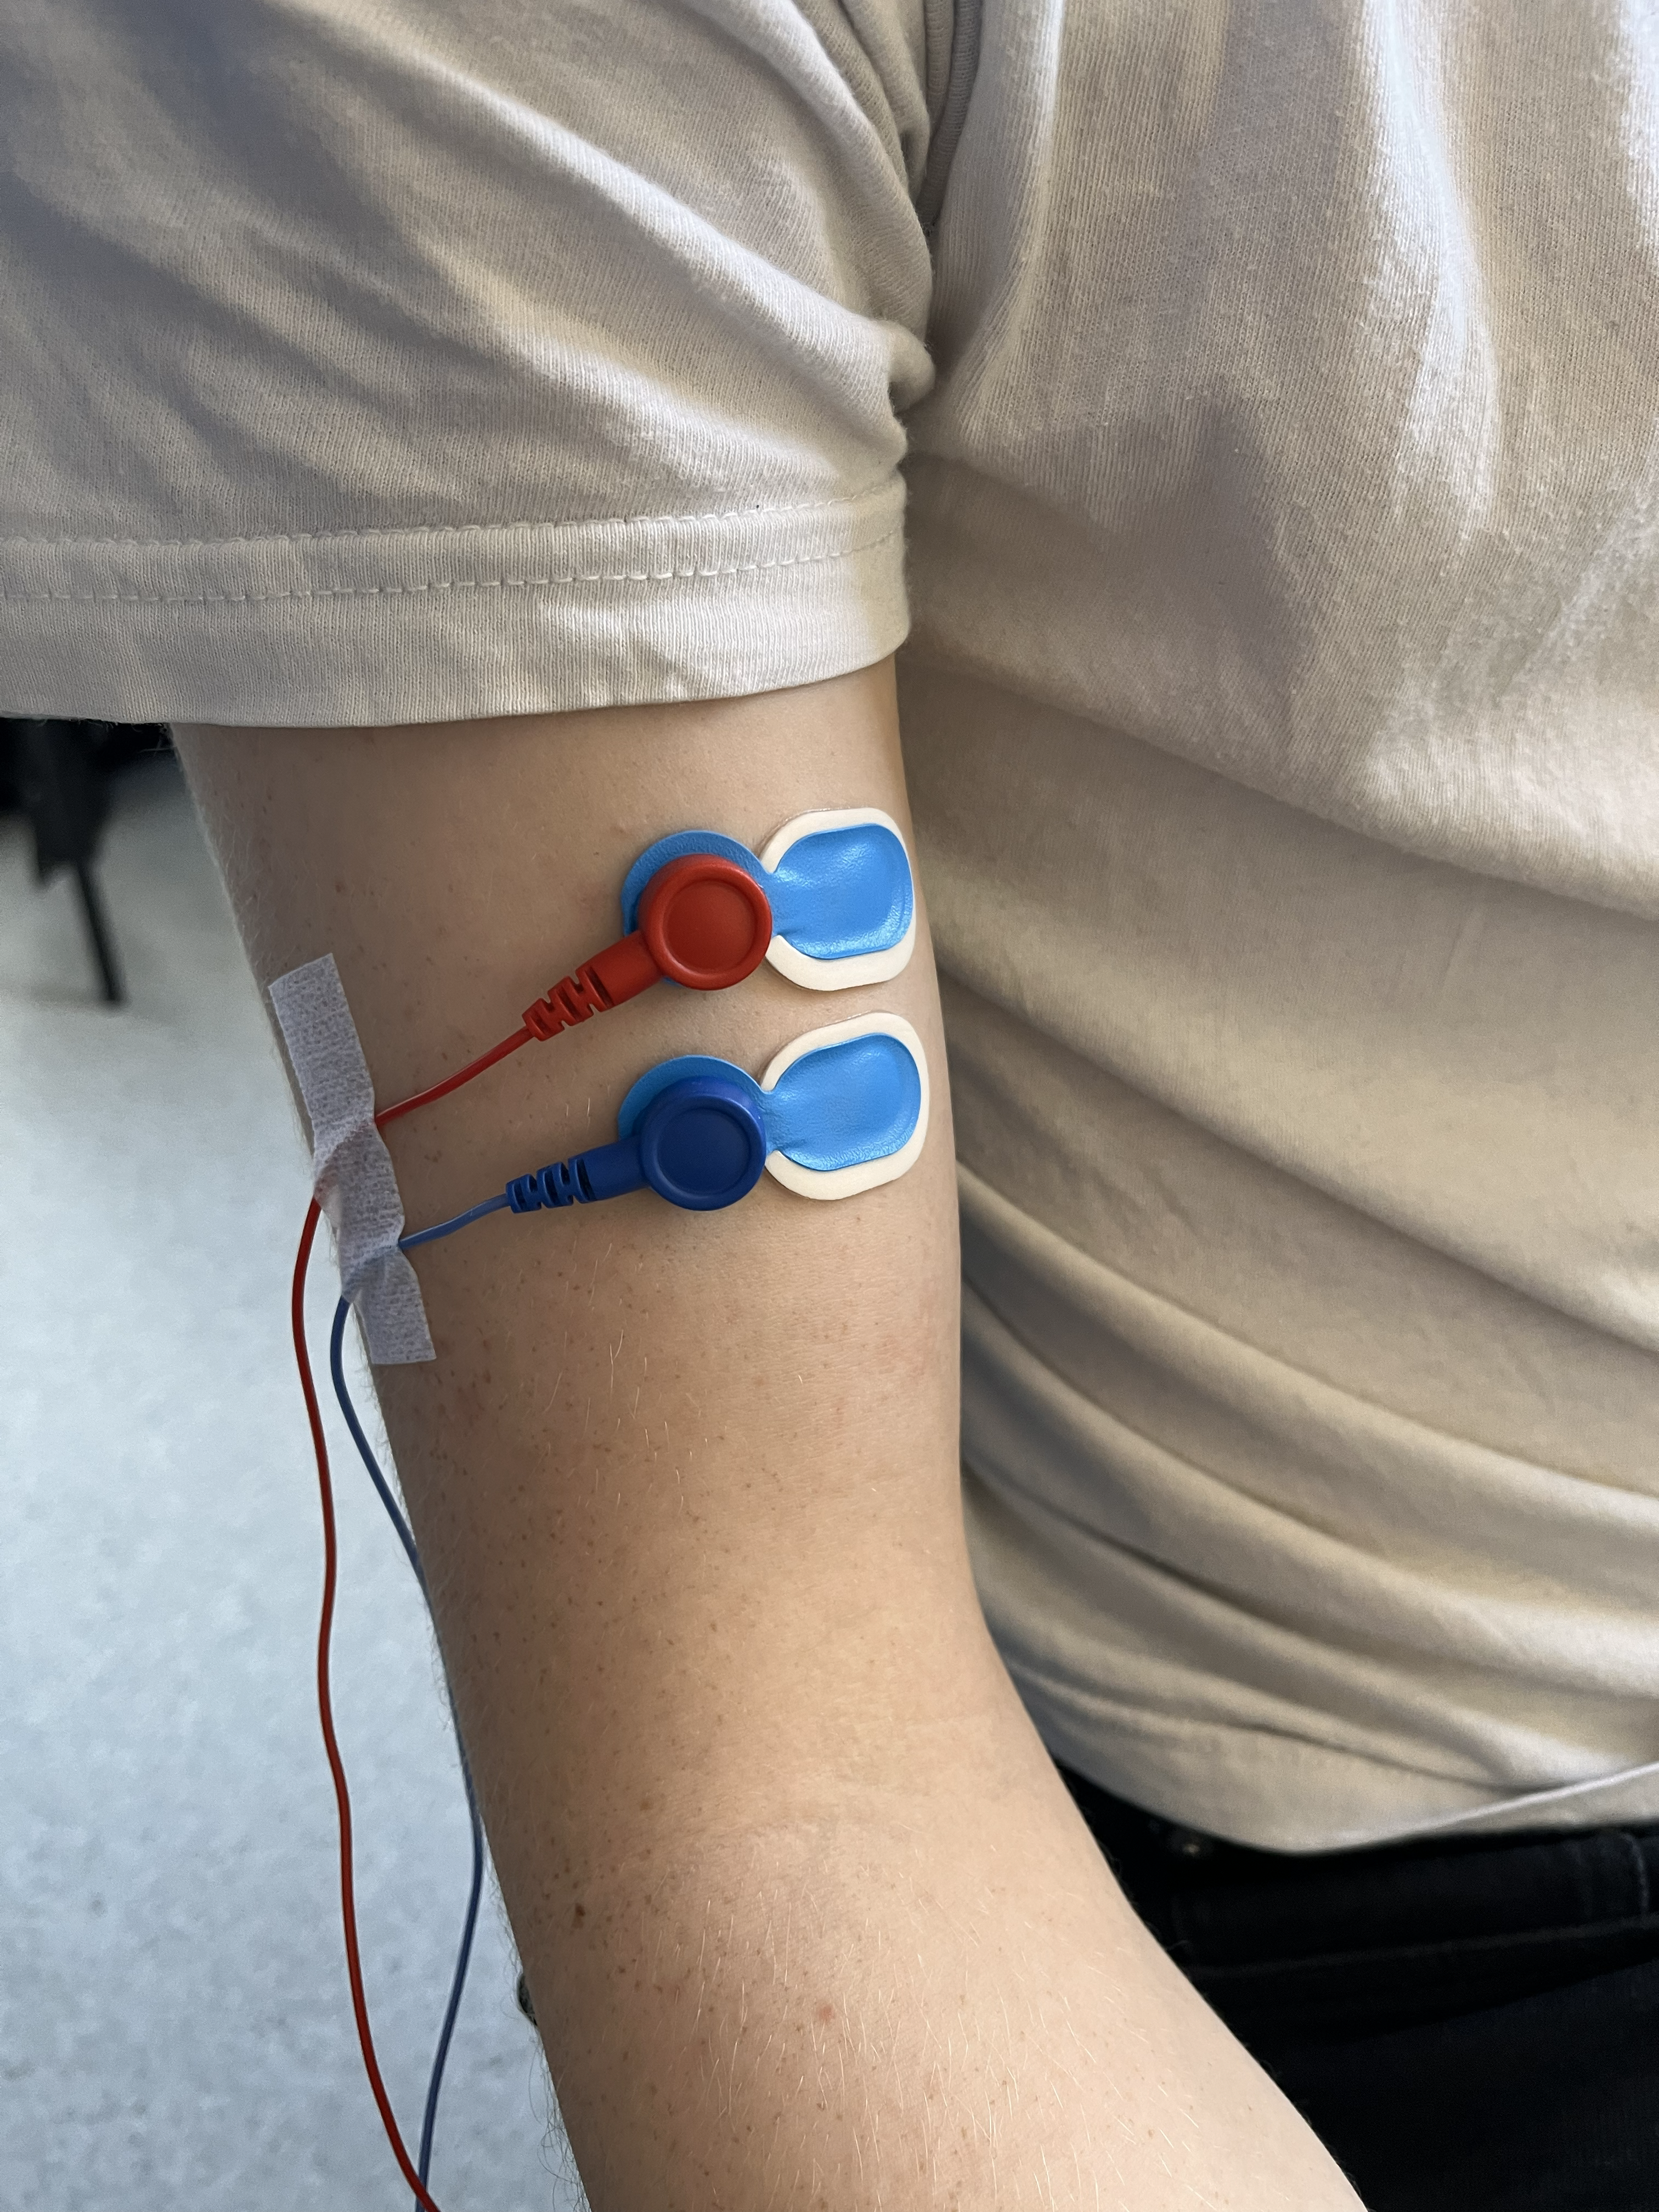
\includegraphics[width=0.3\textwidth]{figures/measuring_electrodes.png}
    \caption{Platzierung der Messelektroden für den MVC-Versuch}
    \label{fig:measuring_electrodes}
\end{figure}

\begin{figure}[h]
    \centering
    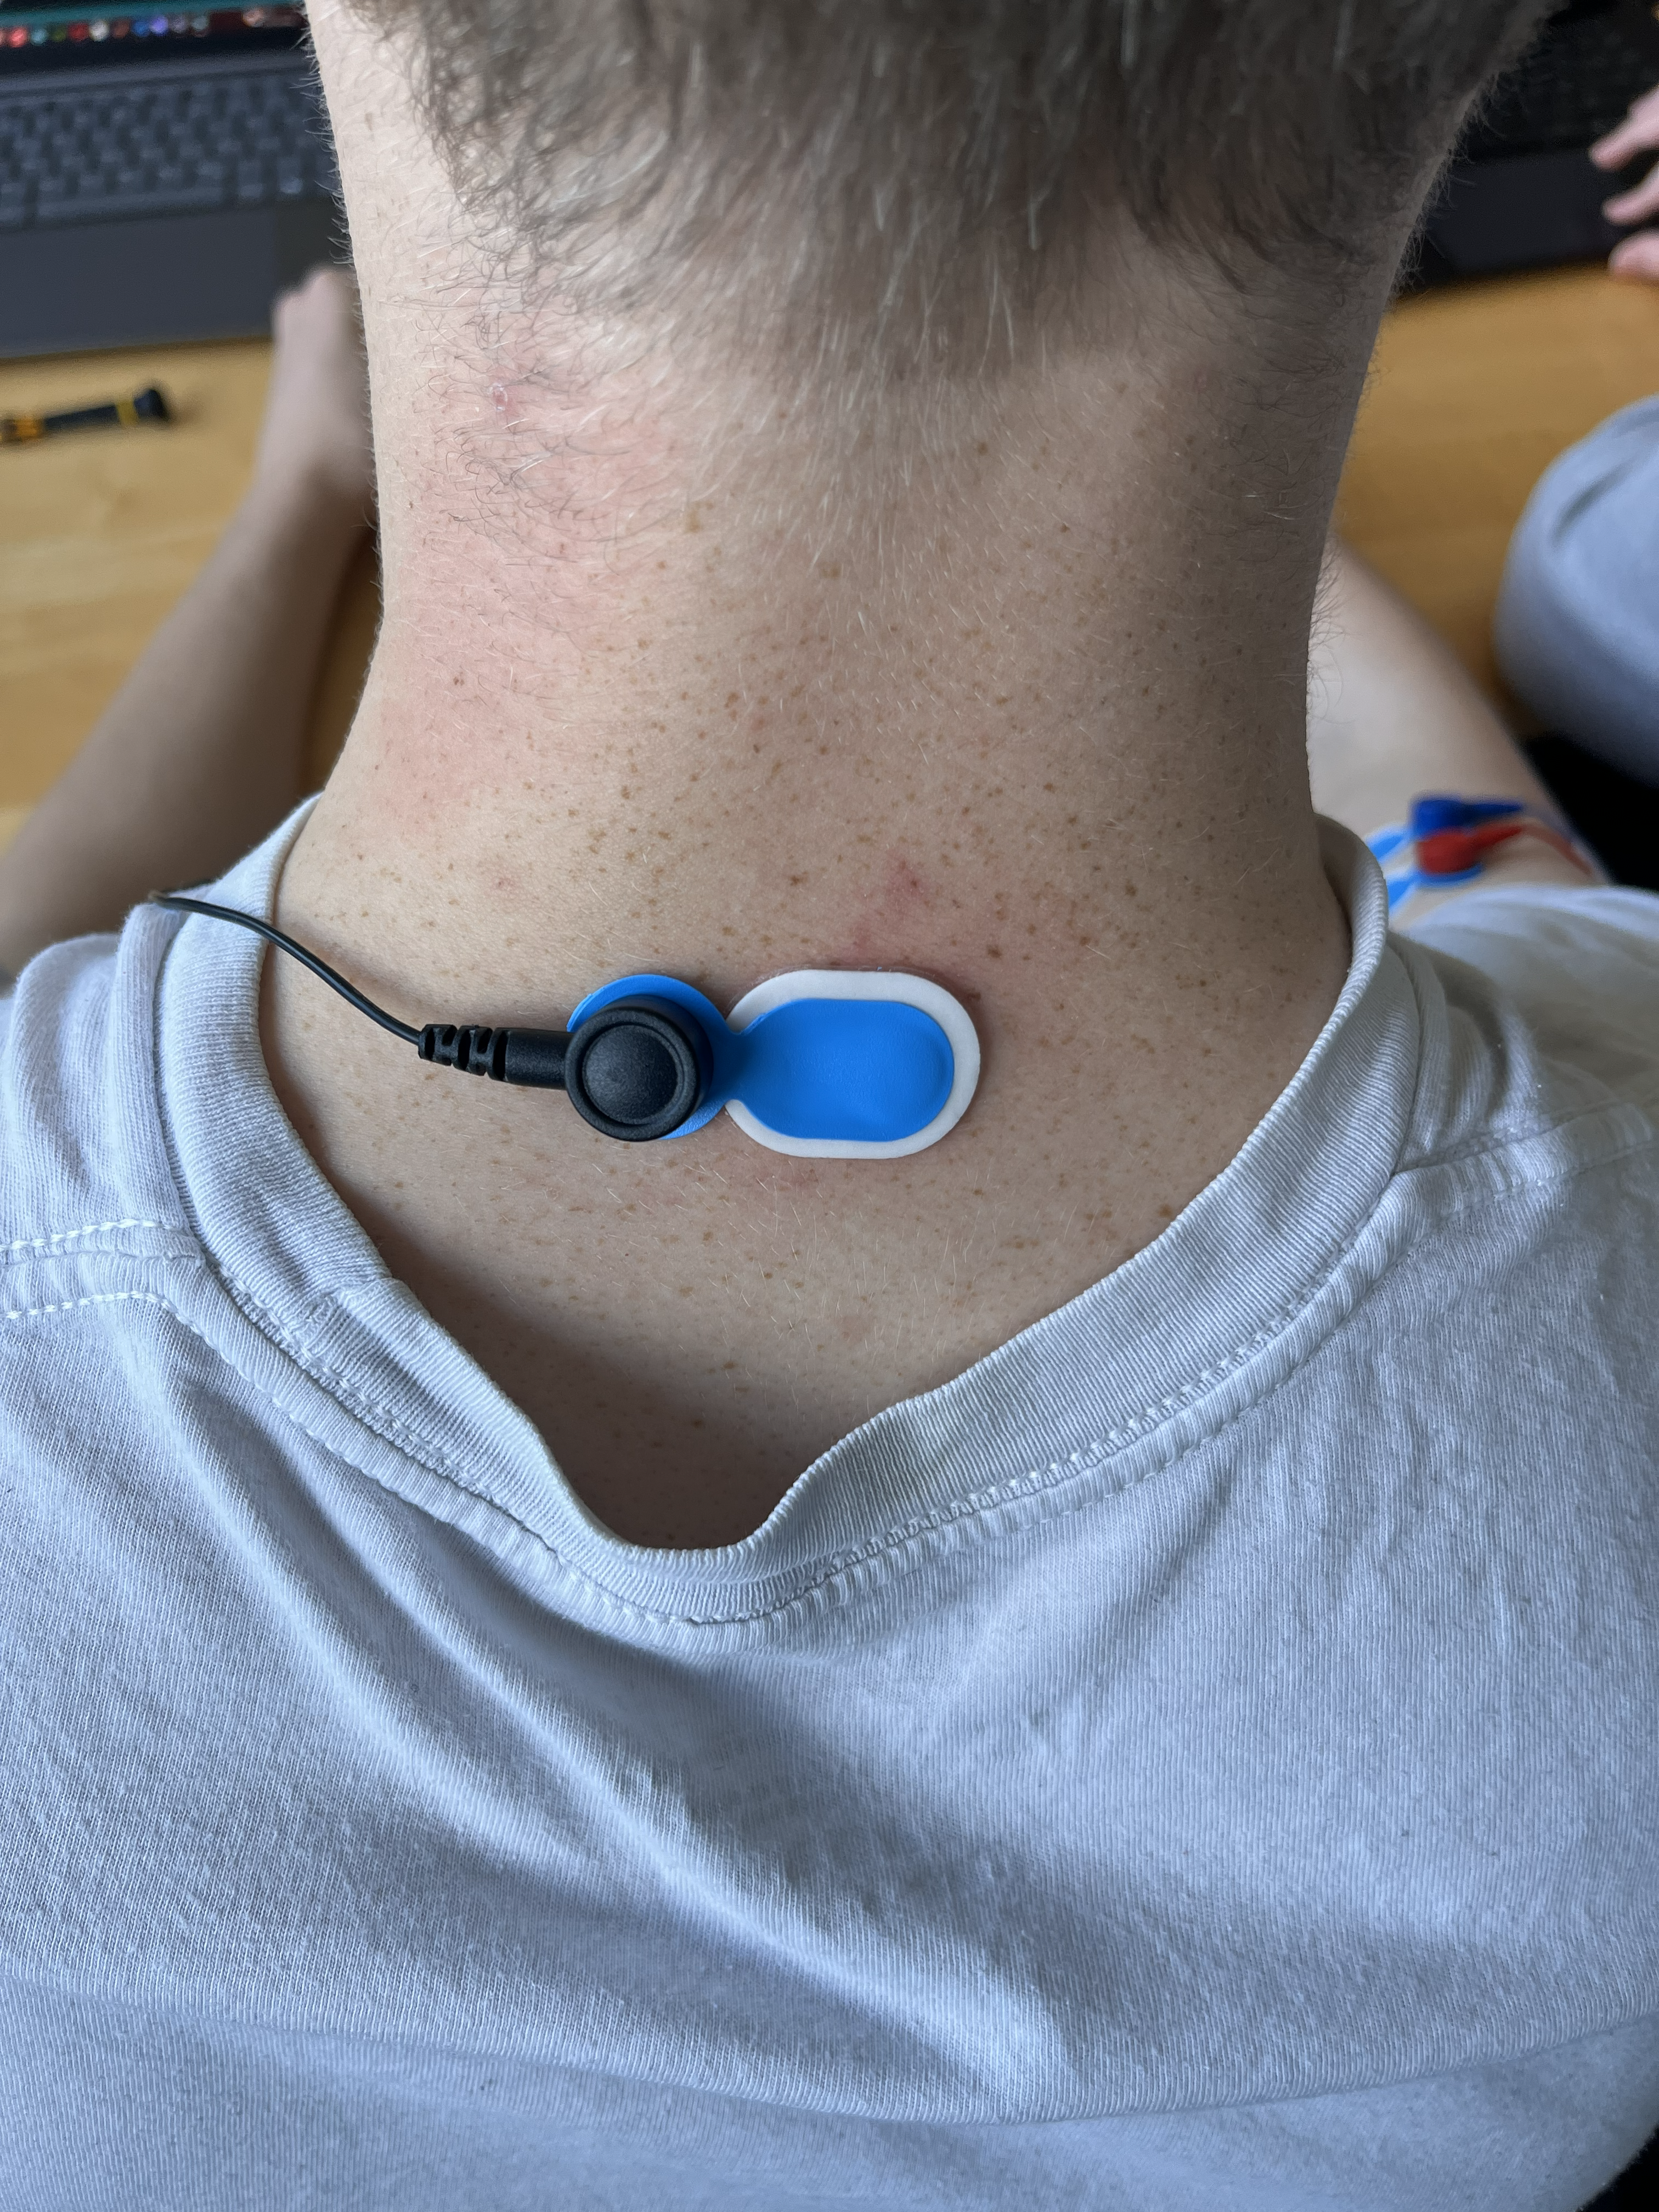
\includegraphics[width=0.3\textwidth]{figures/GND_electrode_c7.png}
    \caption{Platzierung der GND-Elektrode auf dem C7-Wirbel}
    \label{fig:GND_electrode_c7}
\end{figure}

Wie in Abbildung \ref{fig:biceps_tension} zu erkennen ist, sitzt der Proband auf einem Stuhl, wobei der 
Unterarm auf dem Oberschenkel aufliegt. Dadurch stellt sich mit minimaler Bewegung ein etwa 90°-Winkel 
zwischen Ober- und Unterarm ein. Das Handgelenk liegt an der Unterkante des Tisches an. Zur Bestimmung der 
maximalen willkürlichen Kontraktion wird der Proband angewiesen, mit maximaler Kraft zu versuchen, den 
Tisch anzuheben. Gleichzeitig sitzt eine weitere Person auf dem Tisch, um sicherzustellen, dass dieser 
unbeweglich bleibt und keine sichtbare Bewegung stattfinden kann.
\begin{figure}[h]
    \centering
    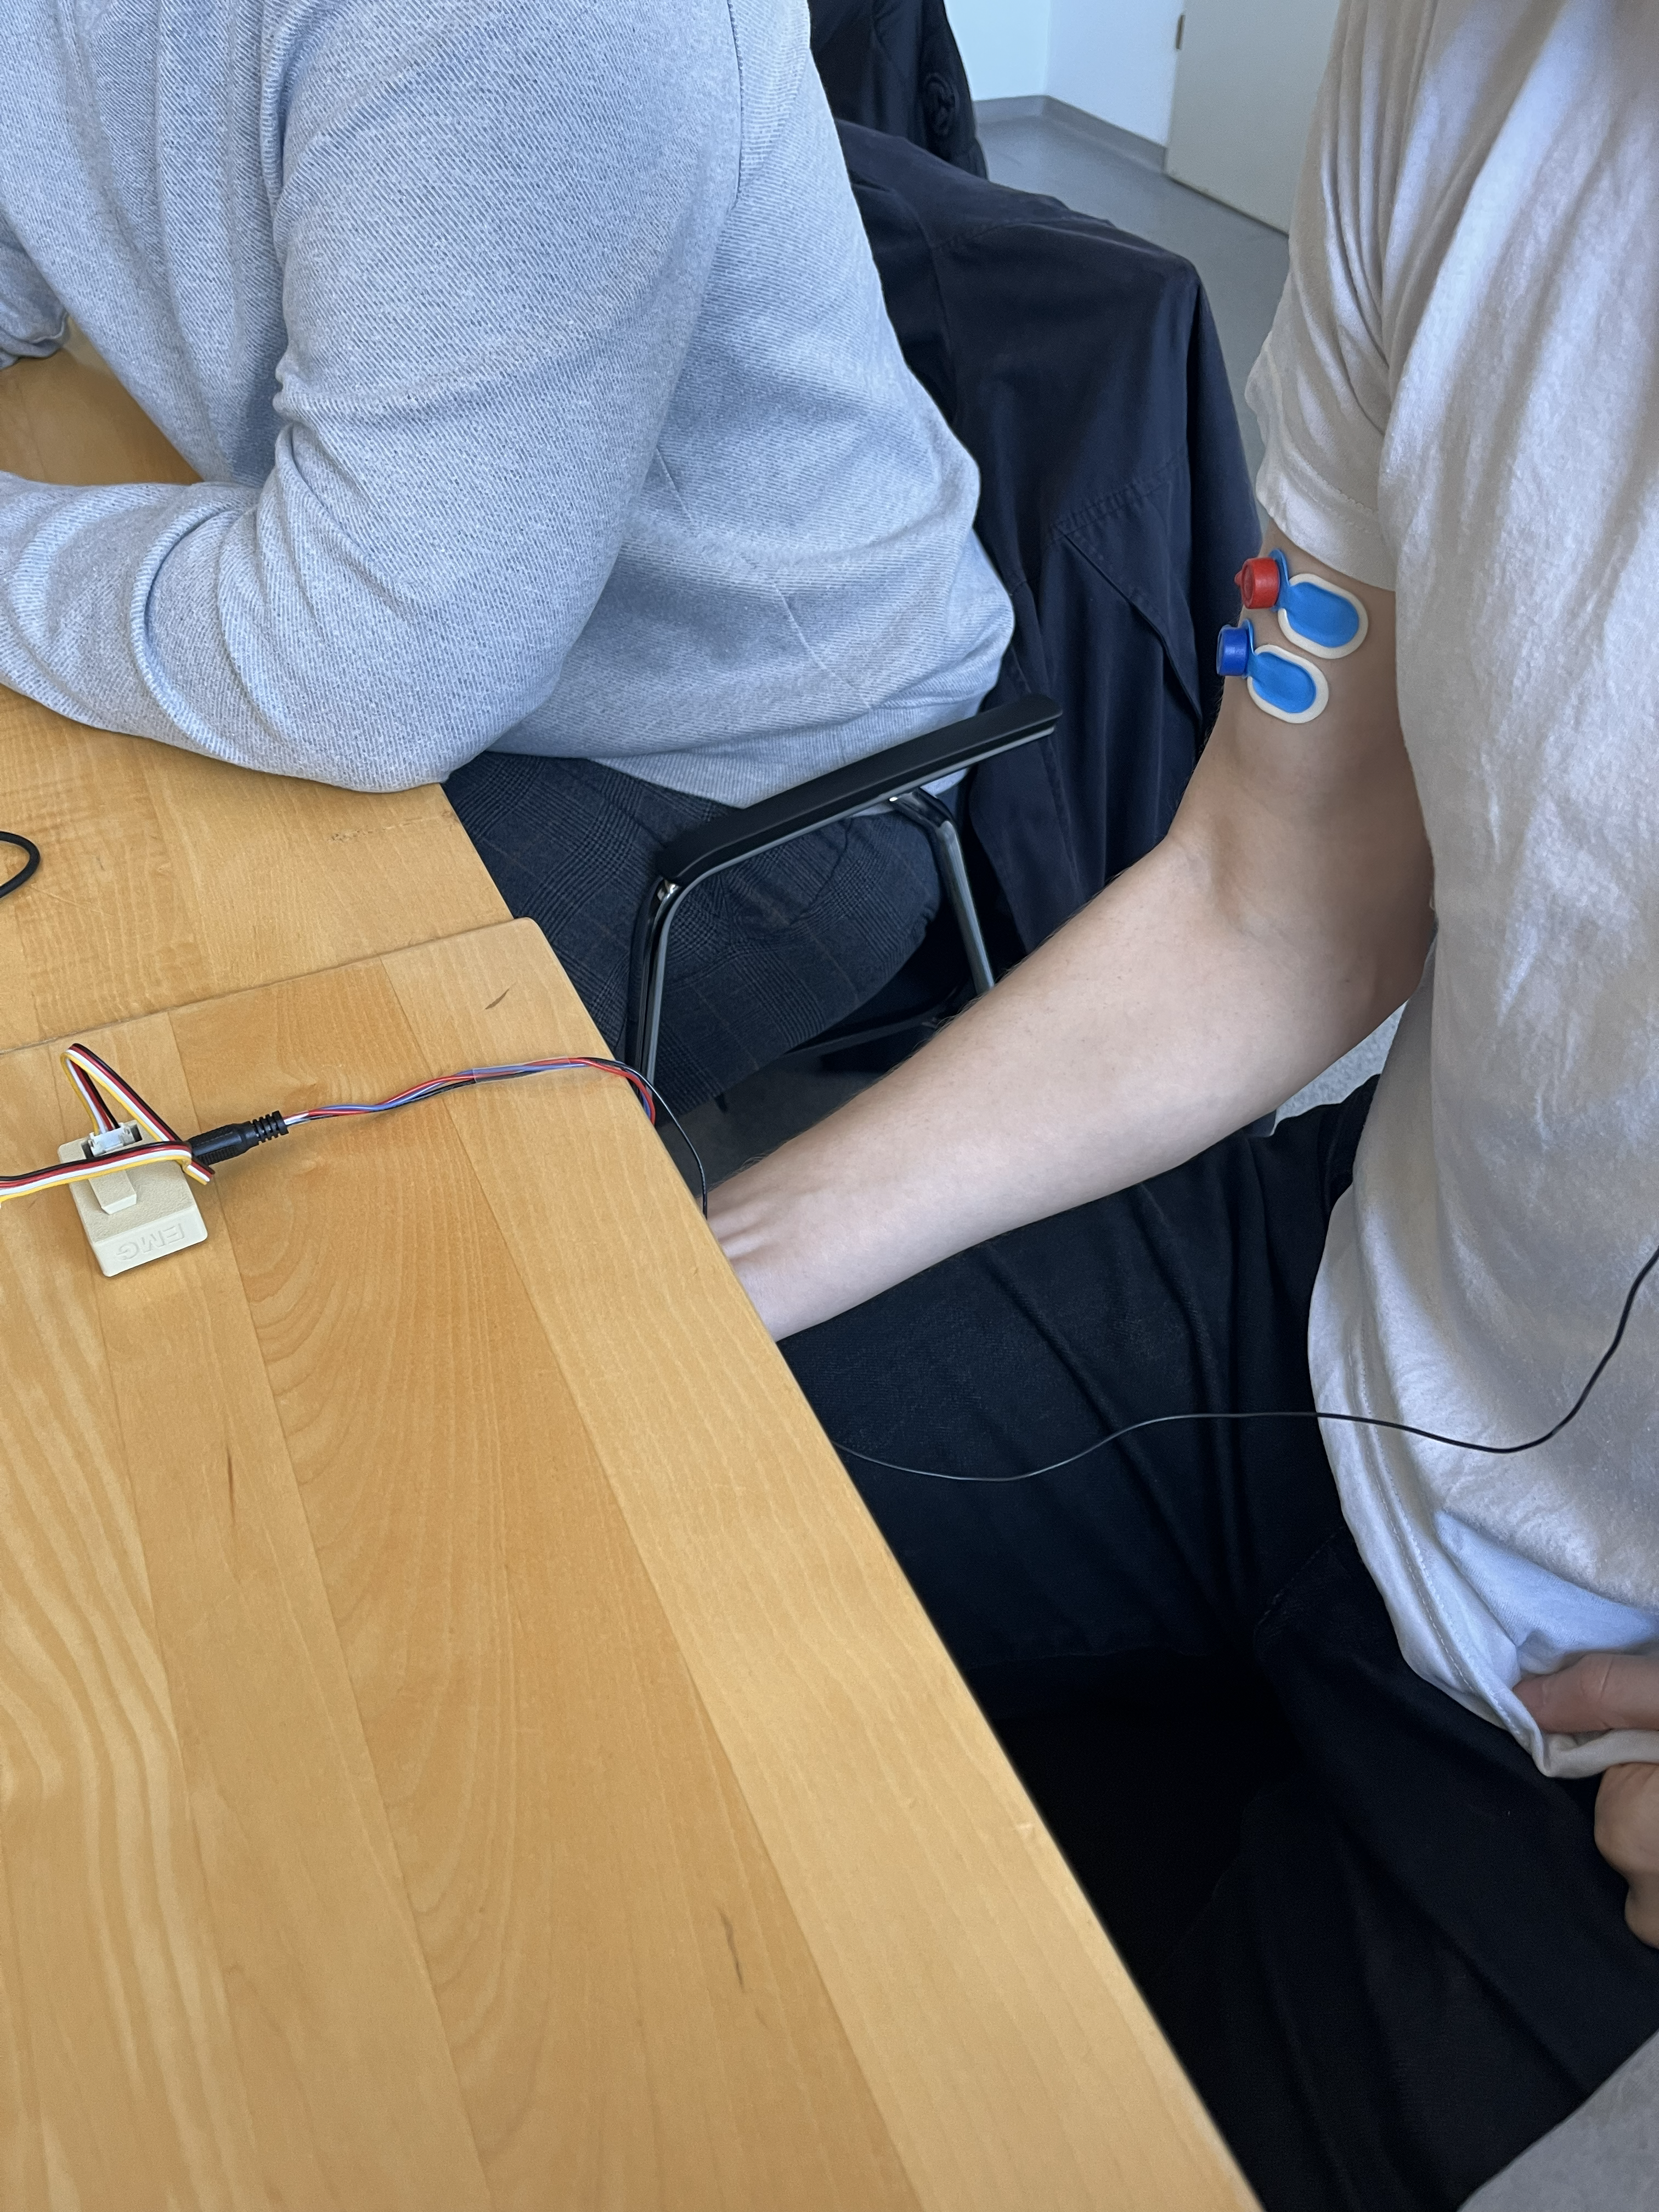
\includegraphics[width=0.4\textwidth]{figures/biceps_tension.png}
    \caption{Angespannter Zustand des Bizeps während des MVC-Versuchs}
    \label{fig:biceps_tension}
\end{figure}
Durch diesen Versuchsaufbau wird eine isometrische Kontraktion des Bizeps brachii ermöglicht, 
bei der der Muskel Kraft entwickelt, ohne sich zu verkürzen. Die gewählte Gelenkstellung von 90° zwischen dem Ober- und Unterarm begünstigt zudem 
eine nahezu optimale Länge-Spannungs-Relation des Muskels. In Kombination mit der stabilen Körperhaltung 
und dem unbeweglichen Widerstand erlaubt dies eine maximale Rekrutierung motorischer Einheiten und somit 
eine maximale willkürliche Kontraktion.
Die maximale Anspannung wird für acht bis zehn Sekunden gehalten, während die EMG-Daten aufgezeichnet 
werden. Dieser Vorgang wird dreimal wiederholt, wobei zwischen den einzelnen Versuchen eine Pause von etwa
einer Minute eingehalten wird, um muskuläre Ermüdung zu vermeiden. Der MVC-Versuch wurde für alle drei 
Gruppenmitglieder durchgeführt.

\subsection{Aufgabe 5: Experiment 2 - Relative Muskelaktivierung}
\begin{figure}[h]
    \centering
    \includegraphics[width=0.6\textwidth]{../Labor_3/data_analysis/mvc_weights.png}
    \caption{Angespannter Zustand des Bizeps während des MVC-Versuchs}
    \label{fig:mvc_weights}
\end{figure}
Zur Bestimmung der maximalen willkürlichen Kontraktion (MVC) wurden die drei MVC-Messungen 
zunächst gemittelt. Mithilfe der Einhüllenden der EMG-Signale konnten die Aktivierungsphasen
eindeutig identifiziert und zeitlich abgegrenzt werden. Innerhalb dieser Intervalle wurde 
der Mittelwert der Muskelaktivierung berechnet und anschließend über alle drei Durchläufe 
gemittelt. Der so ermittelte Wert stellt die individuelle maximale willkürliche Kontraktion 
dar und dient im Folgenden als Referenzgröße.
Wie in Abbildung \ref{fig:mvc_weights} dargestellt, ist bei den Belastungsversuchen eine 
deutlich geringere Muskelaktivierung im Vergleich zur MVC zu beobachten. Die gemessene 
Aktivität liegt erwartungsgemäß bei einem Bruchteil der maximalen willkürlichen Kontraktion.
Dies deutet darauf hin, dass für das Halten submaximaler Gewichte lediglich ein Teil der 
verfügbaren motorischen Einheiten rekrutiert werden muss.
Darüber hinaus zeigt sich, dass die Muskelaktivierung nicht strikt proportional zur 
aufgebrachten Last ansteigt. Dieses Verhalten lässt darauf schließen, dass neben der 
reinen Last weitere Einflussfaktoren, wie die muskuläre Mechanik, die 
Länge-Spannungs-Relation sowie neuronale Steuerungsmechanismen, eine wesentliche Rolle bei 
der Kraftentwicklung spielen.


\subsection{Aufgabe 6: Experiment 3 - Ermüdung}
\begin{figure}[h]
    \centering
    \includegraphics[width=\textwidth]{../Labor_3/data_analysis/frequenzanalyse.png}
    \caption{Frequenzanalyse des EMG-Signals während des Ermüdungsexperiments}
    \label{fig:frequency_analysis_fatigue_experiment}
\end{figure}
In Abbildung \ref{fig:frequency_analysis_fatigue_experiment} ist die Frequenzanalyse des EMG-Signals
während des Ermüdungsexperiments dargestellt. Wir haben uns hier bewusst für die Darstellung der drei Fatigue-Durchläufe entschieden,
um die Konsistenz der beobachteten Veränderungen zu verdeutlichen.

\subsection{Aufgabe 7: Diskussion des Leistungsspektrums}
Wie in Abbildung \ref{fig:frequency_analysis_fatigue_experiment} dargestellt, zeigt das Leistungsspektrum des EMG-Signals eine 
deutliche Konzentration der spektralen Anteile im niedrigen Frequenzbereich.
Dieses Spektralverhalten ist charakteristisch für EMG-Signale während isometrischer Kontraktionen und 
statischer Haltearbeit. Entsprechend liegt auch die Medianfrequenz des Leistungsspektrums im unteren 
Frequenzbereich. Dies weist auf eine dominante Aktivierung von Typ-I-Muskelfasern (Slow-Twitch-Fasern) 
hin, die aufgrund ihrer geringen Kontraktionsgeschwindigkeit und hohen Ermüdungsresistenz besonders für 
ausdauernde Belastungen geeignet sind.
Da das statische Halten eines Gewichts über einen längeren Zeitraum eine Ausdauer- und keine 
Schnellkraftbelastung darstellt, ist die niedrige Medianfrequenz physiologisch plausibel. Veränderungen 
der Medianfrequenz im zeitlichen Verlauf können nach Merletti \cite{Merletti1999SENIAM_SignalProcessing} somit als geeigneter Indikator für muskuläre 
Ermüdungsprozesse herangezogen werden, da eine Abnahme der Medianfrequenz typischerweise mit einer 
Reduktion der Muskelfaserleitgeschwindigkeit einhergeht.

\subsection{Aufgabe 8: Medianfrequenz des Leistungsspektrums}
\begin{figure}[h]
    \centering
    \includegraphics[width=0.6\textwidth]{../Labor_3/data_analysis/median_frequencies.png}
    \caption{Analyse der Medianfrequenz des EMG-Signals während des Ermüdungsexperiments}
    \label{fig:median_frequencies}
\end{figure}

In Abbildung \ref{fig:median_frequencies} ist die zeitliche Entwicklung der 
Medianfrequenz des EMG-Signals während des Ermüdungsexperiments dargestellt.
Es zeigt sich eine kontinuierliche Abnahme der Medianfrequenz im Verlauf der
statischen Haltearbeit.
Dieser Trend gilt als typisches Indiz für muskuläre Ermüdung, da eine Abnahme
der Medianfrequenz mit einer Reduktion der Muskelfaserleitgeschwindigkeit 
assoziiert ist, wie schon in Aufgabe 7 erläutert wurde. Physiologisch lässt sich dieses Verhalten unter anderem 
durch die Akkumulation von Metaboliten, Veränderungen des intrazellulären 
pH-Werts sowie eine Abnahme der Entladungsfrequenz motorischer Einheiten 
erklären. Insbesondere schnell kontrahierende Muskelfasern ermüden im 
Verlauf der Belastung schneller und tragen zunehmend weniger effektiv zur 
Kraftentwicklung bei.
Die beobachtete Verschiebung des Frequenzspektrums zu niedrigeren Frequenzen
bestätigt somit die Annahme, dass während des statischen Halteversuchs 
fortschreitende muskuläre Ermüdungsprozesse auftreten.
\newline
Die Abbildung \ref{fig:median_frequencies} sieht nicht ident aus zu der auf Sakai.
Die Abweichungen zwischen dem dargestellten Diagramm und dem Referenzbeispiel 
lassen sich durch mehrere Faktoren erklären.
EMG-Frequenzparameter unterliegen einer hohen interindividuellen 
Variabilität. Unterschiede in der Muskelfaserzusammensetzung, der neuronalen 
Ansteuerung und dem Ermüdungsverhalten können dazu führen, dass die 
Medianfrequenz zwischen einzelnen Versuchen unterschiedlich verläuft. Darüber
hinaus basiert die Auswertung lediglich auf drei relativen Zeitpunkten, 
wodurch kurzfristige Schwankungen nicht abgebildet werden können. Insgesamt 
zeigt das Diagramm jedoch den erwarteten Trend einer abnehmenden 
Medianfrequenz und bestätigt das Auftreten muskulärer Ermüdung.